\section{Introduction}
\label{sec:introduction}

Techniques for dynamic dependency analysis have been fruitful, with applications ranging from information-flow security~\cite{sabelfeld03} and optimisation~\cite{kildall73} to debugging and program comprehension~\cite{weiser81,delucia96}. There are, however, few methods suitable for fine-grained analysis of richly structured outputs, such as data visualisations and multidimensional arrays. Dataflow analyses \cite{reps95} tend to focus on analysing variables rather than parts of structured values. Where-provenance~\cite{buneman01} and related data provenance techniques are fine-grained, but are specific to relational query languages. Taint tracking \cite{newsome05} is also fine-grained, but works forwards from input to output. For many applications, it would be useful to be able to focus on a particular part of a structured output, and have an analysis isolate the input data pertinent only to that substructure.

This is a need that increasingly arises outside of traditional programming. Journalists and data scientists use programs to compute charts and other visual summaries from data, charts which must be interpreted by colleagues, policy makers and lay readers alike. Interpreting a chart correctly means understanding what the components of the visualisation actually \emph{represent}, i.e.~the mapping between data and visual elements. But this is a hard task, requiring time and expertise, even with access to the data and source code used to create the visualisation. In practice it is easy for innocent (but devastating) mistakes such as transposing two columns of data to go unnoticed~\cite{miller06}. Since visualisations are simply cases of programs that transform structured inputs (data tables) into structured outputs (charts and other graphics), general-purpose language-based techiques for fine-grained dependency tracking should be able to help with this, by making it possible to reveal these relationships automatically to an interested user.

\subsection{Linking structured outputs to structured inputs}
\label{sec:introduction:data-linking}

First, interpreting a chart would be much easier if the user were able to explore the relationship between the various parts of the chart and the underlying data interactively, discovering the relevant relationships on a need-to-know basis. For example, selecting a particular bar in a bar chart could highlight the relevant data in a table, perhaps showing only the relevant rows, as illustrated in \figref{introduction:data-linking}. We could certainly do more and say something about the nature of the relationship (summation, in this case), but even just revealing the relevant data puts a reader in a much better position to fact-check or confirm their own understanding of what they are looking at. Indeed, visualisation designers sometimes create ``data-linked'' artefacts like these by hand, such as Nadieh Bremer's award-winning visualisation of population density growth in Asian cities~\cite{bremer15}, at the cost of significant programming effort. Libraries such as Altair \cite{vanderPlas18} alleviate some of this work, but require data transformations to be specified using a limited set of combinators provided (and understood) by the library.

\begin{figure}
   \begin{subfigure}[b]{0.99\textwidth}
      \centering
      {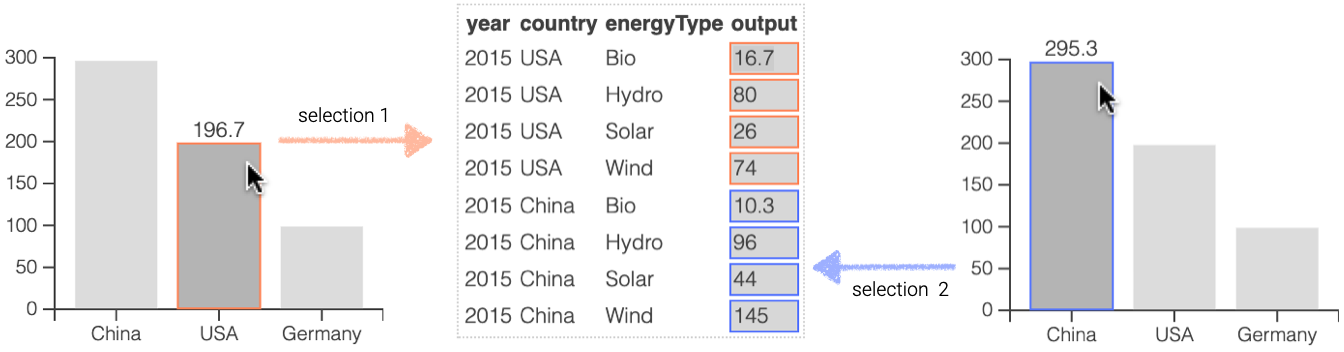
\includegraphics[scale=0.55]{fig/example/data-linking-merged.png}}
   \end{subfigure}\\
   \vspace{2mm}
   \begin{subfigure}{0.65\textwidth}
      \small
      \lstinputlisting[language=Fluid]{fluid/bar-chart.fld.mod}
   \end{subfigure}
   \caption{Fine-grained linking of outputs to inputs, focusing on data for USA (left) and China (right).}
   \label{fig:introduction:data-linking}
\end{figure}

What we would like to do is allow data scientists to author analyses and visualisations using an expressive functional language like the one shown in \figref{introduction:data-linking}, with data linking provided automatically for the computed artefact as a baked-in transparency feature. At the core of this is a program analysis problem: we want to be able to focus on a particular chart element, and determine the inputs that contribute to it. Given the output selection, this is a matter of performing some kind of backwards analysis to identify the relevant data. As well as providing a path to automation, framing data linking as a program analysis problem invites interesting questions that a hand-crafted solution is unlikely to properly address. For example, does the union of two output selections depend on the union of their respective dependencies? Do dependencies ``round-trip'', in that they identify sufficient resources to reconstruct the selected output? Are they minimal? These questions are important to establishing trust and a language-based approach offers a chance to address them.

\subsection{Linking structured outputs to other structured outputs}
\label{sec:introduction:vis-linking}

Second, authors often present distinct but related aspects of data in separate charts. In this situation a reader should be able to focus on (select) a visual element in one chart or other structured output and automatically see elements of a different chart which were computed using related inputs. For example in \figref{introduction:vis-linking} below, selecting the bar on the left should automatically highlight all the related visual elements on the right. This is a well-recognised use case called \emph{brushing and linking}~\cite{becker87}, which is supported by geospatial applications like GeoDa~\cite{anselin06} and charting libraries like Plotly, but tends to be baked into specific views, or require programmer effort and therefore anticipation in advance by the chart designer. Moreover these applications and libraries provide no direct access to the common data which explains why elements are related.

\begin{figure}
  \begin{subfigure}[b]{0.99\textwidth}
     \centering
     {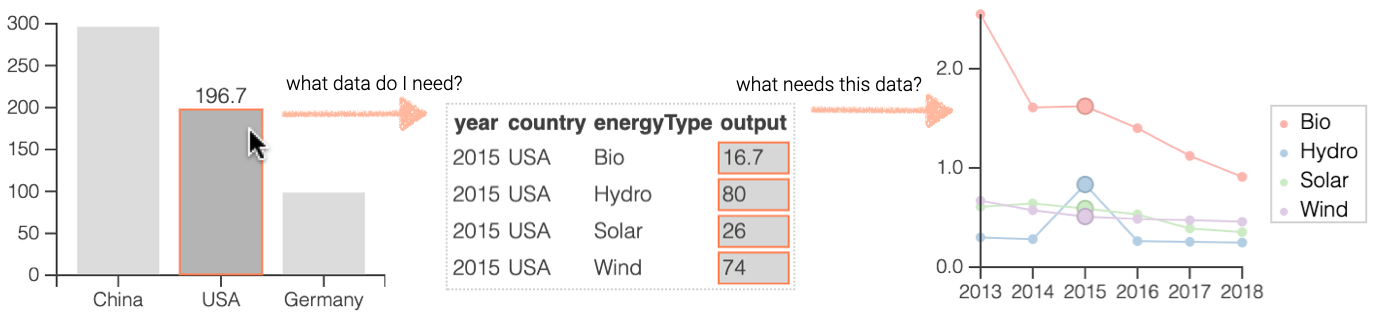
\includegraphics[scale=0.58]{fig/example/vis-linking.png}}
  \end{subfigure}\\[2mm]
  \begin{subfigure}{0.8\textwidth}
     \small
     \lstinputlisting[language=Fluid]{fluid/line-chart.fld.mod}
  \end{subfigure}
 \caption{Linking visualisations via common data dependencies}
 \label{fig:introduction:vis-linking}
\end{figure}

Again, we would like to enable a more automated (and ubiquitous) version of brushing and linking, without imposing a burden on the programmer. They should be able to express visualisations and other data transformations using standard functional programming features such as those shown in \figref{introduction:vis-linking}, and have brushing and linking enabled automatically between computed artefacts which depend on common data. At the core of this requirement is a variant of our original program analysis problem: we want to select a part of the output and perform a backwards analysis to identify the required inputs, as before, but then also to perform a forwards analysis to identify dependent parts of the other output. Moreover, we would also like the brushing and linking feature to be able to provide a concise view of the data that explain why the two selections are linked. Note that the intuition behind the forwards analysis here is not the same as the one we appealed to in the context of round-tripping: there the (hypothetical) question was whether the selected data was \emph{sufficient} to reconstruct the selected output, whereas to identify related items in another view, we must determine those parts for which the selected data is \emph{necessary}. As before, a language-based approach offers the prospect of addressing these sorts of question in a robust way.

\subsection{Contributions}

To make progress towards these challenges, we present a bidirectional analysis which tracks fine-grained data dependencies between input and output selections, with round-tripping properties characterised by Galois connections. Selections have a complement, which we use to adapt the analysis to compute fine-grained dependencies between two outputs which depend on common inputs. Recent program slicing techniques~\cite{perera12a,perera13a,ricciotti17} allow the user to focus on the output by ``erasing'' parts deemed to be irrelevant; the erased parts, called \emph{holes}, are propagated backwards by a backwards analysis which identifies parts of the program and input which are no longer needed. Although these approaches also enjoy useful round-tripping properties characterised by Galois connections, they only allow focusing on \emph{prefixes} of a structured output, rather than arbitrary substructures, a notion which is not closed under complement. Our specific contributions are as follows:

\begin{itemize}
   \item[--] a new bidirectional dynamic dependency analysis which operates on selections of arbitrary parts of data values, for a core calculus with lists, records and mutual recursion, and a proof that the analysis is a Galois connection (\secref{data-dependencies});
   \item[--] a second bidirectional dependency analysis, derived from the first by De Morgan duality, which is also a Galois connection and which can be composed with the first analysis to link outputs to outputs, with an extended example based on matrix convolution  (\secref{de-morgan});
   \item[--] a richer surface language called \OurLanguage, implemented in PureScript, with familiar functional programming features such as piecewise definitions and list comprehensions, and a further Galois connection linking selections between the core and surface languages (\secref{surface-language}).
\end{itemize}

\noindent First we introduce the core calculus which provides the setting for the rest of the paper, and which will serve as the desugaring target for the surface syntax presented in \secref{surface-language}.
